\documentclass[12pt, a4paper]{article}

\usepackage[utf8]{inputenc}
\usepackage[T1]{fontenc}
\usepackage[english]{babel}
\usepackage{booktabs}
\usepackage{graphicx}
\usepackage{microtype}
\usepackage{parskip}

\title{Reproducibility of Chaos Experiments in Ecoscape}
\date{}

\begin{document}

\maketitle

\subsection*{Implementation}

Ecoscape is implemented as a Kubernetes-native operator that relies on two external
dependencies: \textbf{Prometheus} for metrics collection and SLO evaluation, and
\textbf{Chaos Mesh} for fault injection. The entire benchmark configuration is expressed
declaratively through three Custom Resource Definitions (CRDs):
\texttt{Topology}, \texttt{ChaosPhase}, and \texttt{Experiment}.

\textbf{Topology.}
The \texttt{Topology} CRD describes the logical structure of the edge environment.
Each zone represents an isolated network domain with configurable resource limits ---
CPU, memory, and storage --- reflecting the hardware constraints of real edge devices.
Connections between zones are declared as \emph{links} and model realistic WAN
characteristics such as latency, jitter, bandwidth, and packet loss.
The topology can be activated and deactivated, so that network conditions are selectively
applied for the duration of an experiment while the deployed system environment is
preserved.

\textbf{ChaosPhase.}
The \texttt{ChaosPhase} CRD defines a reusable fault scenario that is specified
independently of any concrete experiment. A fault scenario consists of one or more
fault definitions referencing named zones of the associated topology. Supported fault
types include network-based faults (latency, bandwidth, packet loss, partitioning) as
well as resource-based faults (CPU and memory stress), covering typical stress scenarios
encountered in edge operation. Additionally, arbitrary platform-specific fault scenarios
can be integrated via a generic extension mechanism.

\textbf{Experiment.}
The \texttt{Experiment} CRD is the central orchestration resource. It references a
\texttt{Topology} and a \texttt{ChaosPhase}, and defines the benchmark lifecycle:
following a configurable warm-up phase, a baseline measurement is conducted without
active faults, succeeded by a chaos measurement phase with injected faults. This cycle
is executed for a configurable number of repetitions. System quality is assessed through
\emph{Service Level Objectives} (SLOs), declared as PromQL expressions with associated
thresholds. Ecoscape thus constitutes a \textbf{performance resilience benchmark for
edge computing}, enabling reproducible experiments that are fully described declaratively
and executed under realistic edge network conditions.

\subsection*{Experiment Setup}

To assess the reproducibility of Ecoscape, the following SUT was simulated within the framework.

The System under Test is an \textbf{edge sensor pipeline} consisting of three logical zones:
two edge zones (\texttt{zone1}, \texttt{zone2}) and one fog zone. Each edge zone runs a
Redis instance acting as a local stream buffer, and a simulated sensor producer that
continuously writes readings to the local Redis Stream. The fog zone hosts an aggregator
service that maintains a consumer group per zone, continuously reading from both edge
Redis instances and exposing aggregated metrics via Prometheus.

The topology is declared as a \texttt{Topology} CR and defines baseline network conditions
as links: fog $\leftrightarrow$ zone1 at 30\,ms / 3\,ms jitter (fibre uplink),
fog $\leftrightarrow$ zone2 at 50\,ms / 5\,ms jitter (LTE), and zone1 $\leftrightarrow$
zone2 at 15\,ms / 2\,ms jitter.

The injected fault is defined as the \texttt{ChaosPhase} \textbf{esp-stress-cloud}, which
applies 80\,\% CPU stress on the fog zone, simulating compute pressure on the aggregator.

The \texttt{Experiment} CR references the topology and the ChaosPhase. The lifecycle runs
for \textbf{8 repetitions}, each consisting of a warm-up phase, a 90\,s pre-chaos baseline
measurement, fault injection, and a 90\,s chaos measurement window, followed by a recovery
pause. System quality is assessed through two SLOs, both measuring Redis stream consumer
group lag --- \texttt{stream-lag-zone1} and \texttt{stream-lag-zone2} --- with a threshold
of 50 unconsumed messages.

\subsection*{Reproducibility of Chaos Experiments}

To assess the impact of the injected chaos fault on each SLO, two complementary
descriptive metrics are reported across the eight experimental repetitions.

\textbf{Relative effect size ($\delta$).} For each repetition, the relative change
between the pre-chaos baseline and the chaos phase is computed as
$\delta = (\mu_{\text{chaos}} - \mu_{\text{pre}}) / \mu_{\text{pre}}$,
where $\mu$ denotes the per-phase mean. This scale-normalised metric enables a
direct comparison between SLOs that operate at different absolute value ranges.
The mean and standard deviation of $\delta$ across all repetitions characterise
both the magnitude and the consistency of the observed effect.

\textbf{Absolute dispersion on a common scale.} The per-repetition chaos-phase
means are normalised to the global value range observed across both SLOs combined.
The standard deviation of these normalised means quantifies run-to-run variability
on a shared reference scale, making both groups directly comparable regardless of
their differing absolute magnitudes.

\begin{table}[h]
\centering
\caption{Summary of relative effect size and absolute dispersion across eight
         repetitions per SLO.}
\label{tab:reproducibility}
\begin{tabular}{lcccccc}
\toprule
\textbf{SLO} & \textbf{mean($\delta$)} & \textbf{std($\delta$)} &
\textbf{min($\delta$)} & \textbf{max($\delta$)} &
\textbf{std (norm.)} & \textbf{CV (norm.)} \\
\midrule
stream-lag-berlin & $+1.48$ & $1.53$ & $-0.32$ & $+4.56$ & $0.016$ & $0.67$ \\
stream-lag-munich & $+25.83$ & $10.52$ & $+7.19$ & $+41.49$ & $0.133$ & $0.50$ \\
\bottomrule
\end{tabular}
\end{table}

\textbf{Results and discussion.}
For \texttt{stream-lag-munich}, the chaos fault produces a large and consistently
positive effect across all eight repetitions (mean $\delta = +25.83$,
std $= 10.52$). The minimum observed effect ($\delta = +7.19$) confirms that
Munich's stream lag increases substantially in every single run.
On the normalised scale, per-repetition means range from $0.11$ to $0.49$
(std $= 0.133$), reflecting variation in magnitude but not in direction.

For \texttt{stream-lag-berlin}, the picture is more nuanced. In absolute terms,
Berlin's values remain negligibly small across all runs (std$_{\text{norm}} =
0.016$), staying consistently near zero relative to the global measurement range.
However, the relative effect size reveals a small but non-negligible average
increase (mean $\delta = +1.48$, std $= 1.53$), with one repetition even showing a
marginal decrease ($\delta = -0.32$). This suggests that the chaos fault does
induce minor fluctuations in Berlin's stream lag, even if the absolute impact
remains far below Munich's.

\textbf{Reproducibility.}
The Ecoscape experiments demonstrate reproducibility at the level of qualitative
outcome: \texttt{stream-lag-munich} is consistently and substantially affected by
the injected fault in all eight repetitions, while \texttt{stream-lag-berlin}
remains unaffected in absolute terms. However, full quantitative reproducibility
cannot be claimed. The Munich effect varies considerably in magnitude across runs
(CV $= 0.50$), which is an inherent characteristic of chaos experiments involving
non-deterministic fault injection. Berlin's relative effect, while small on
average, also shows high variability (CV $= 1.03$ on $\delta$), with individual
repetitions occasionally producing non-trivial changes. These observations
suggest that while the Ecoscape framework reliably discriminates between affected
and unaffected SLOs, the precise magnitude of the chaos effect is subject to
run-to-run variation and should be interpreted with caution.

Figure~\ref{fig:chaos_combined} visualises both SLOs on a shared time axis and
y-axis. The shaded bands represent the min/max range (lightest), the mean\,$\pm$\,std
interval (medium), and the median (solid line) across all eight repetitions.
The dashed vertical line separates the pre-chaos baseline from the chaos phase.

\begin{figure}[h]
\centering
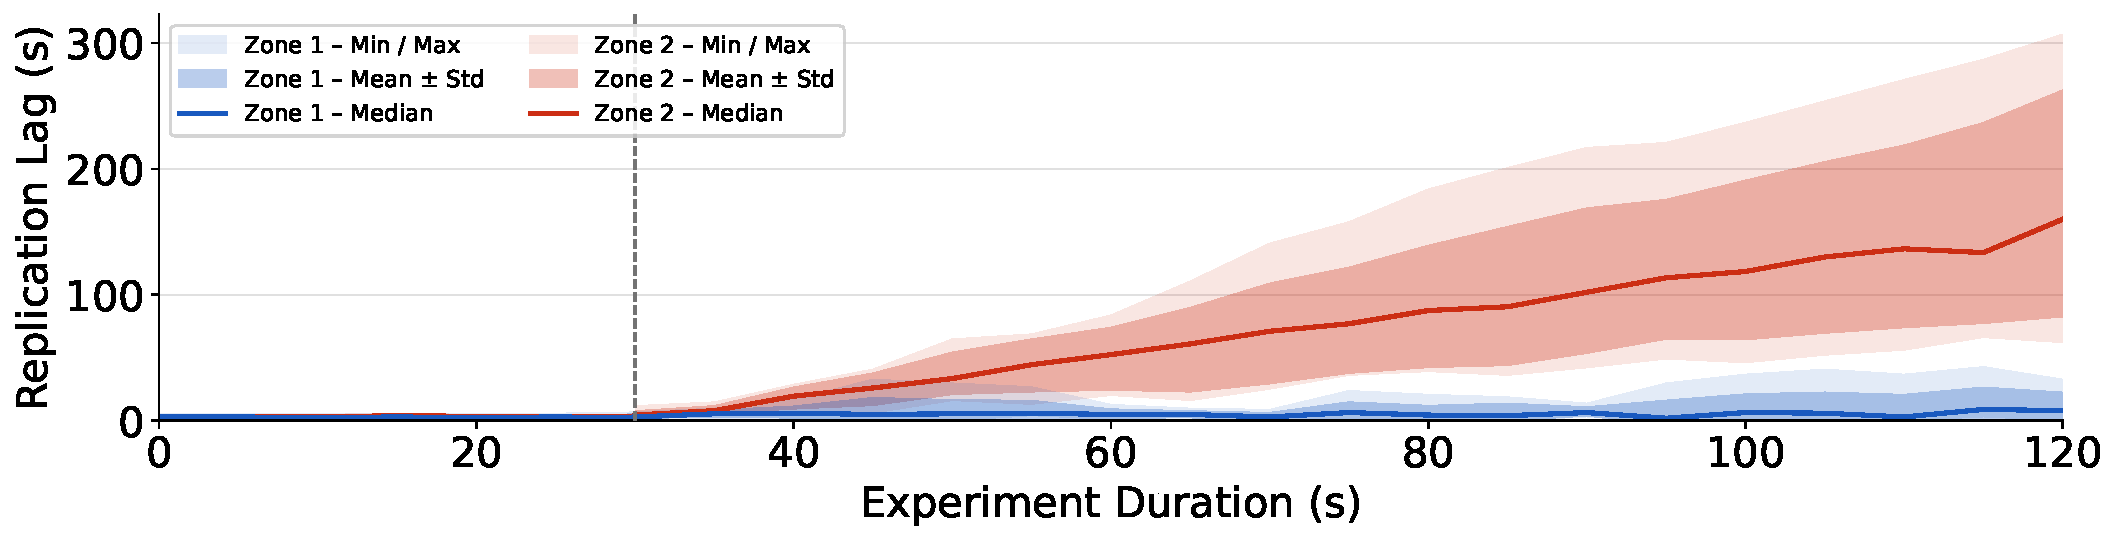
\includegraphics[width=\linewidth]{chaos_effect_combined.pdf}
\caption{Combined view of \texttt{stream-lag-munich} (red) and
         \texttt{stream-lag-berlin} (blue) over time. Shaded bands show
         min/max (light) and mean\,$\pm$\,std (medium) across eight repetitions;
         solid lines show the median. The dashed line marks the transition from
         pre-chaos baseline to chaos phase.}
\label{fig:chaos_combined}
\end{figure}

\end{document}
